%!TEX root = thesis.tex
\todo{Note that this is a conceptual prototype, not an actual implementation} 
For our first prototype description we will dig into the area of shape changing interfaces, SCIs.
We will do this to explore and illustrate the possibilities of creating AHIs based on shape-change.
More specifically we will touch upon a specific approach to constructing SCIs called jamming.
SCIs were introduced in the introduction of this thesis as interfaces that use physical change of shape as input or output.
Jamming is special kind of technique that can be used to control the stiffness of a material which makes it possible to construct objects that can change their surface structure.
What makes SCIs interesting to AHIs is it''s ability to dynamically change the physical properties of an interface element, be it shape, texture, stiffness, position ect.
This change in physicality can then be the offset for a new temporary interaction possibility that is created for the specific situation, where afterwards it can return to it''s initial natural state.
This aspect aligns well with the definition of AHIs that we presented earlier in section \todo{ref to AHI section} 

\section{Jamming as an enabling technology}
\label{ch:jamming:enabling-technology} 
%!TEX root = ../thesis.tex
Before continuing on the topic of jamming, let's first give an introduction to the mechanics of jamming.

Jamming is a mechanism that can enable granular material to transition between solid-like and liquid-like states. These states can occur if the material is put under an external stress, figure~\ref{fig:ch:jamming:phase-transition} illustrate these states.
Much like water can shift to gas when heated and to ice when cooled. But where water is affected by thermodynamics, granular systems are not. \hl{entirely true?}
Sand, which is a granular material, may resemble a liquid as it flows through an hour glass, although the individual grains themselves are a solid structure. This is due to something called \todo{Jamming, Force chains and Fragile matter}

\begin{figure}[hb]
	\centering
  		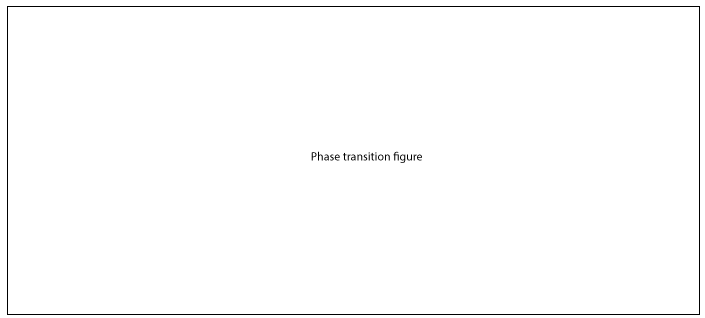
\includegraphics[width=4in]{figures/jamming/phase_transition}
	\caption[Phase transition from \textit{liquid} state to \textit{solid} state.]
   {Phase transition from \textit{liquid} state to \textit{solid} state.}
   \label{fig:ch:jamming:phase-transition}
\end{figure}

You might have noticed how some coffee packagings at the local super market are like a rigid container, see figure~\ref{fig:ch:jamming:coffee-packaging}. 
In this kind of packaging, after filling it with coffee, all excess air has been sucked out by applying a vacuum, i.e. jamming the coffee grains, and thereby making it almost rock solid. 
Also, think about a regular bean bag which exhibits some of the same properties, see figure~\ref{fig:ch:jamming:bean-bag}. 
When no force is applied to it, i.e. no one is sitting in it, it resembles the liquid-like state mentioned earlier. 
When a person then sits down in a bag air will be pressed out and the particles (most often polystyrene foam) will be pushed tightly together filling the voids  \todo{some physical term here, phase space and stuff} thereby jamming the particles making it resemble a solid ...

\begin{figure}
\centering
\begin{minipage}[t]{.5\textwidth}
  \centering
  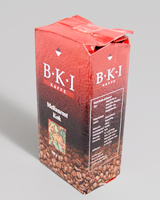
\includegraphics[width=.4\linewidth]{figures/jamming/coffee_packaging}
  \captionof{figure}{Coffee in vacuum packaging}
  \label{fig:ch:jamming:coffee-packaging}
\end{minipage}%
\begin{minipage}[t]{.5\textwidth}
  \centering
  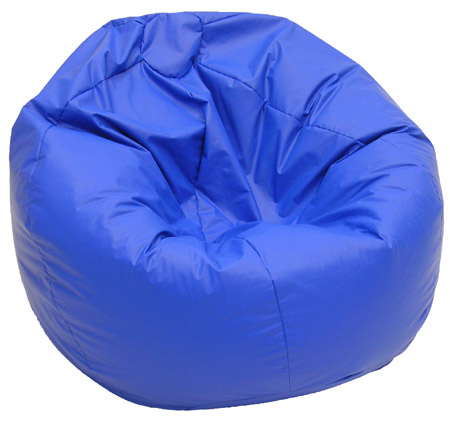
\includegraphics[width=.4\linewidth]{figures/jamming/bean_bag}
  \captionof{figure}{A bean bag}
  \label{fig:ch:jamming:bean-bag}
\end{minipage}
\end{figure}

\subsection{Particles}
\label{ch:jamming:particles}
The granular material, also called the particles, can be any material that has the physical properties that allow for jamming to occur. 
But parameters such as particle size, shape and compressibility have an impact on the jamming transition. 
This has been investigated by several researchers, e.g. \cite{cheng2012design} and \cite{steltz2010jamming}, where the stress to strain ratio \todo{explain this} of different granular materials are evaluated. 
Ground coffee (fine and coarse) and glass beads of varying size are recurring across these tests, the first being an irregular shape with a rough surface as opposed to the plain shape and smooth surface of the second, see figure~\ref{fig:ch:jamming:particles-close-up}. 
Particles of same size and with a smooth surface will tend to be more fluid-like when unjammed as they flow more freely. 
Irregular particles with rough surfaces will create more friction between the particles thus being less fluid-like in the unjammed state.

The conclusion is that the choice of granular material is very much dependent on the application in question. 

\begin{figure}
\centering
\begin{subfigure}{.5\textwidth}
  \centering
  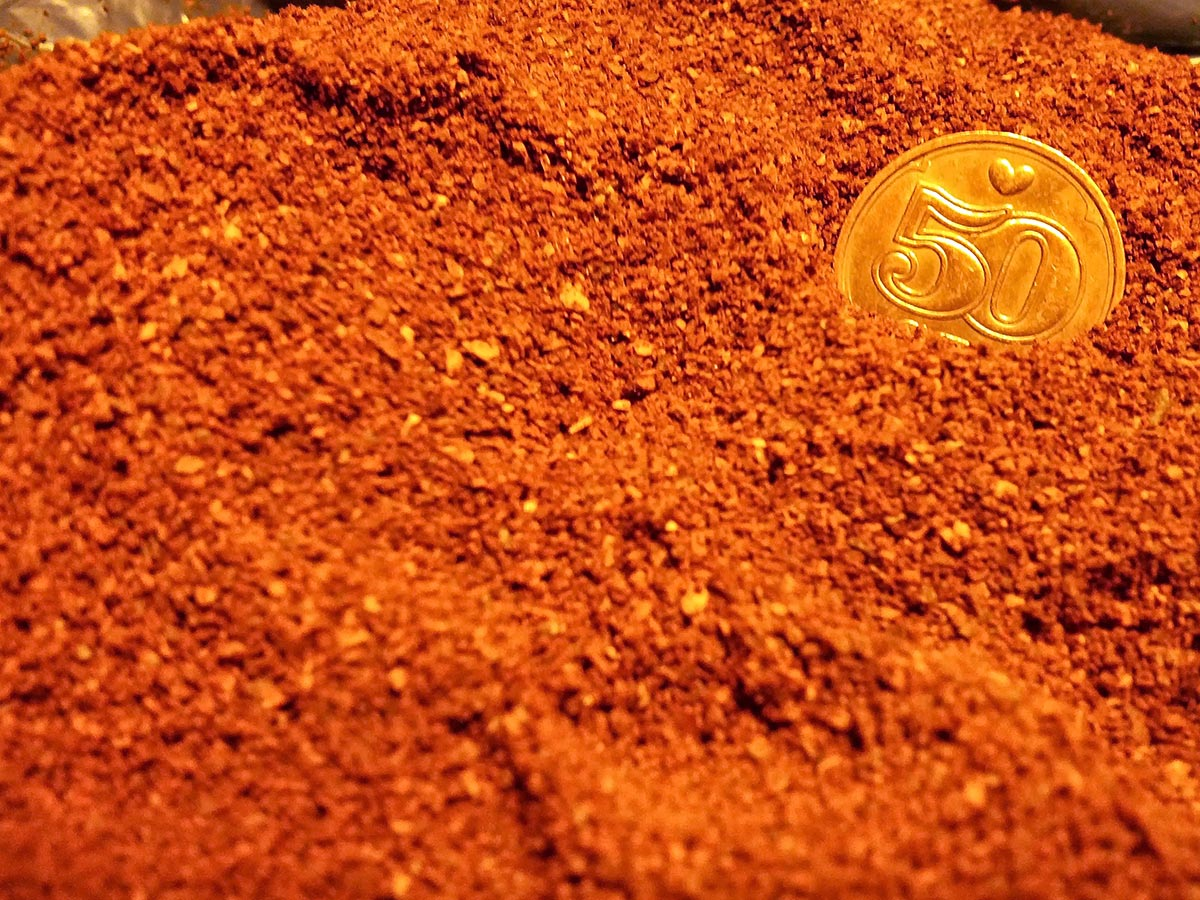
\includegraphics[width=.9\linewidth]{figures/jamming/coffee-grains}
  \caption{Grounded coffee}
  \label{fig:sub1}
\end{subfigure}%
\begin{subfigure}{.5\textwidth}
  \centering
  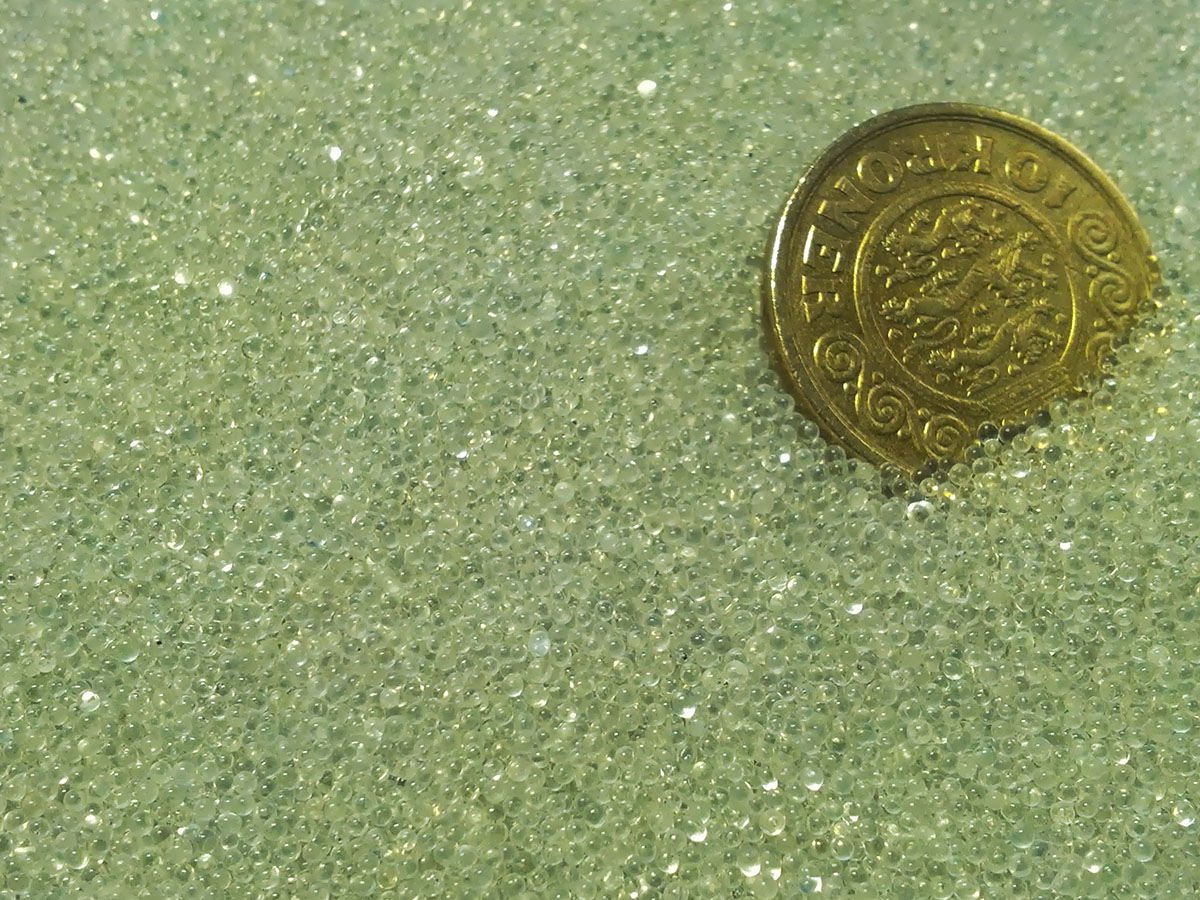
\includegraphics[width=.9\linewidth]{figures/jamming/glass-beads}
  \caption{Glass beads}
  \label{fig:sub2}
\end{subfigure}
\caption{A microscopic view of different granular material.}
\label{fig:ch:jamming:particles-close-up}
\end{figure}

\todo{research in particle parameters in other\\ disciplines such as robotics.}

\begin{itemize}
	\item http://en.wikipedia.org/wiki/Jamming\_(physics)
	\item http://www.nature.com/nphys/journal/v3/n4/full/nphys580.html
	\item http://www.nature.com/nature/journal/v411/n6839/full/411772a0.html
\end{itemize}

\subsection{The technique}
\label{ch:jamming:technique}

The jamming technique can be applied with both a pneumatic and a hydraulic approach.
In the pneumatic approach a gas, for example air, is used as a means for actuation, see figure~\ref{fig:ch:jamming:jamming-basics}.
The gas is enclosed together with granular material within a flexible and air tight container, for example rubber latex. 
A filter prevents the granular material from escaping the container and a valve upholds the pressure.
An external vacuum pump can then suck out the air of the container, creating a negative pressure inside, which results in the transition to a solid-like form. 
The speed of this transition of course depends on the suction power of the pump.
When the vacuum is released the form will gradually transition back to the liquid state. 
In this way, the transition allows for states in between the two extremes; solid and liquid.

Jamming makes it possible to deform an object by hand while in the liquid state and then apply the vacuum and make the deformed object solid - in a sense the form is \emph{saved} as long as the vacuum is maintained.
Figure~\ref{fig:ch:jamming:jamming-transition} shows a transition where a form has been molded and solified into a shape.
When the pressure is released the form gradually changes shape as seen in the individual steps of the figure.
In the setup a balloon was used as the membrane and ground coffee within as particles.
Pressure was applied with a vacuum cleaner and a coffee filter prevents the particles from being sucked out.

In the example it can be seen that the object (balloon) returns to its initial state which is a requirement for SCIs as stated earlier in section \ref{ch:jamming:vocabulary}.
In this example it is the tension of the latex of the balloon that forces it back but it could as well have been an actuation done with the jamming technique itself. 

\begin{figure}[hb]
	\centering
  		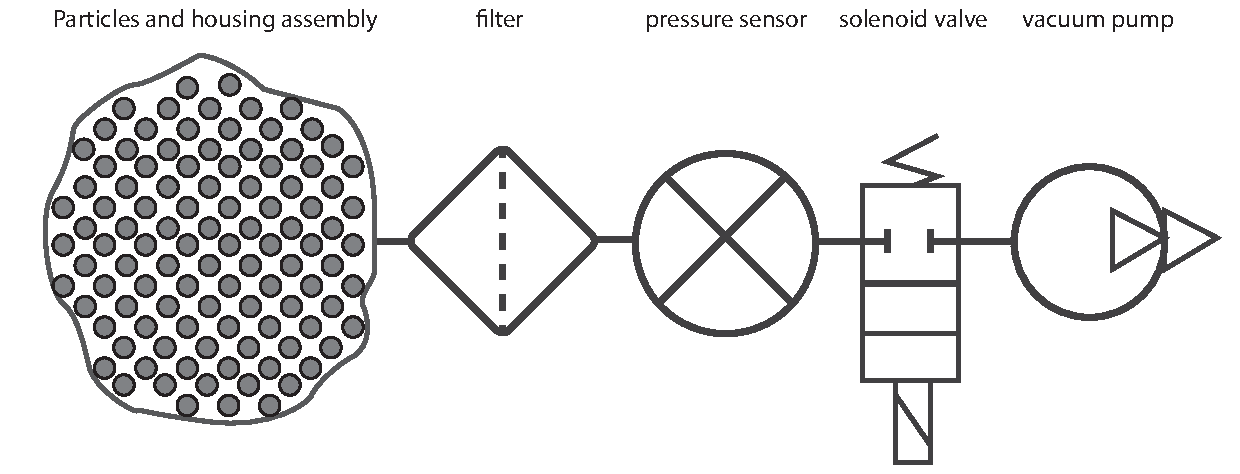
\includegraphics[width=4in]{figures/jamming/jamming-basics}
	\caption[A basic pneumatic jamming system.]
   {A basic pneumatic jamming system.}
   \label{fig:ch:jamming:jamming-basics}
\end{figure}

\begin{figure}[hb]
  \centering
      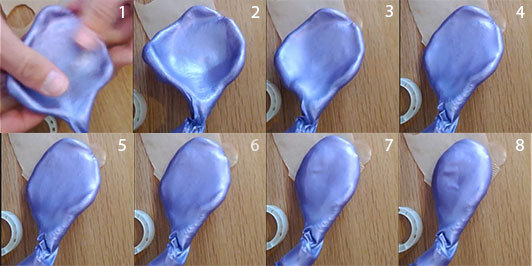
\includegraphics[width=\textwidth]{figures/jamming/jamming-transition}
  \caption[A jamming transition setup.]
   {Jamming transition with a balloon, grounded coffee, vacuum cleaner and a coffee filter.}
   \label{fig:ch:jamming:jamming-transition}
\end{figure}



\section{Related work}
\label{ch:jamming:related-work} 
%!TEX root = ../thesis.tex
Although jamming might seem as a novel approach in the area of HCI, other areas of research have had it on their agenda for some time. 
Especially in the area of mechanical engineering where the jamming mechanism has shown promising results in robotic applications as a substitute for mechanical parts.
In the following we cover the current applications of jamming in both HCI and engineering. 

\subsubsection{Mechanical engineering and robotics}

\citet{brown2010universal} and \citet{amend2012positive} used the jamming technique to develop a universal robotic gripper, which is the tool at the end of a robotic arm that interacts with its environment.
This is an example of the basic jamming approach with a single volume, as in figure~\ref{fig:ch:jamming:approaches:basic}.
The gripper was simply built with an elastic bag as a container for the granular material, which was chosen to be grounded coffee. 
It is able to pick up objects of heterogeneous shapes due to the gripper simply adapting to the surface structure of the objects on impact, see figure~\ref{fig:ch:jamming:jamming-robot-gripper}. 
Contrasting this with a normal mechanical robotic arm which needs several actuators to grap objects of heterogeneous shapes, this gripper is implemented with a single actuator, the jamming volume, which still obtains multiple degrees of freedom (DoF).

\begin{figure}[h]
  \centering
  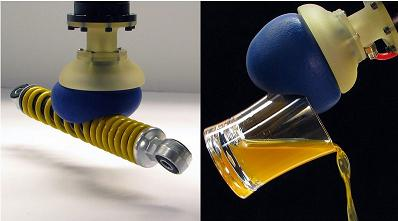
\includegraphics[width=0.9\linewidth]{figures/jamming/jamming-robot-gripper}
	\caption[A universal robotic gripper based on the jamming of granular material by \citet{brown2010universal}.]
   {A universal robotic gripper based on the jamming of granular material \citep{brown2010universal}.}
   \label{fig:ch:jamming:jamming-robot-gripper}
\end{figure}

Jamming is also seen in experiments with autonomous robots where the mechanism can be used as artificial muscles.
\citet{steltz2009jsel} used the jamming technique to create a platform for shape-changing and mobile robots called JSEL (Jamming Skin Enabled Locomotion).
As opposed to the previous example this work is based on the cell-based jamming approach, as seen in \ref{fig:ch:jamming:approaches:cell}.
The soft robot can morph its ``skin'' to create movement of the entire body by controlling the stiffness of the individual cells and inner actuator (see figure~\ref{fig:ch:jamming:jsel}). 

\citet{steltz2010jamming} took the JSEL approach further combining the cell-based approach with a linear actuator. 
The assembly combines the contraction and extension capabilities of the linear actuator and modulates this 1-DoF actuation into a multi-DoF actuator depending on the number of surrounding jamming cells.
The platform is called JMU (Jamming Modulated Unimorph) and has been tested as component segments of a worm, as an example of a soft robot (see figure~\ref{fig:ch:jamming:jmu}).

These different examples from other fields of research illustrate how creative implementations of the jamming technique can substitute mechanical parts and in many ways simplify the implementation.

\begin{figure}
  \centering
  \begin{minipage}[t]{.44\textwidth}
    \centering
    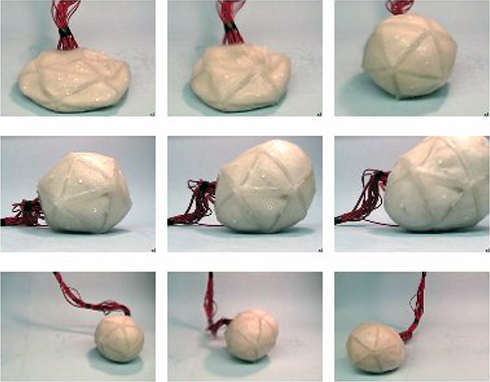
\includegraphics[width=\linewidth]{figures/jamming/chembot-robot-blob}
    \caption[Jamming Skin Enabled Locomotion (JSEL) by \citet{steltz2009jsel}.]
    {Jamming Skin Enabled Locomotion (JSEL). Each cell can be jammed individually to create motion \citep{steltz2009jsel}.}
    \label{fig:ch:jamming:jsel}
    \hspace{.2\textwidth} 
  \end{minipage}%
  \hspace{0.02\textwidth}
  \begin{minipage}[t]{.44\textwidth}
    \centering
    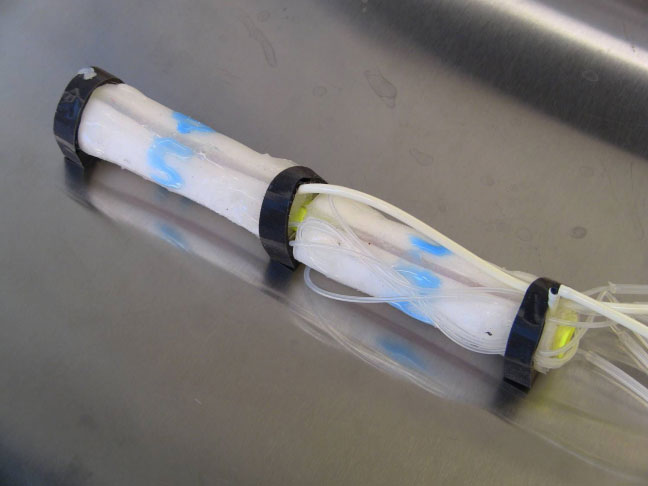
\includegraphics[width=\linewidth]{figures/jamming/jmu-worm}
    \caption[Jamming Modulated Unimorph by \citet{steltz2010jamming}.]
    {Jamming Modulated Unimorph \citep{steltz2010jamming}.}
    \label{fig:ch:jamming:jmu}
  \end{minipage}
\end{figure}

\subsubsection{Human-computer Interaction}
\label{ch:jamming:related-work:hci}
Jamming has also been explored in the area of HCI though to a limited extent.
Most of the examples here are very recent contributions (2012) but they do show promising applications.

\paragraph{Dynamically changeable physically buttons (\citeyear{harrison2009providing})} 
\label{ch:jamming:related-work:hci:dynbuttons}
This first example is actually not based on jamming but on some of the same principles, where pneumatic actuation is used to enable deformations on a latex surface.
The project presents a visual display which contains deformable areas able to create physical buttons.
An acrylic backing layer with cut-out areas for the shapes and positions of the buttons are placed under an upper latex surface.
With pneumatic control it is possible to dynamically make physical buttons appear at the cut-out areas as either convex, concave, or flat forms, see figure~\ref{fig:ch:jamming:concepts:harrisonhudson}.
Though button states can be modified they are still in a very static configuration due to the cut-out areas which cannot be changed.

\begin{figure}[h]
  \centering
  \begin{minipage}[b]{.8\textwidth}
    \centering
    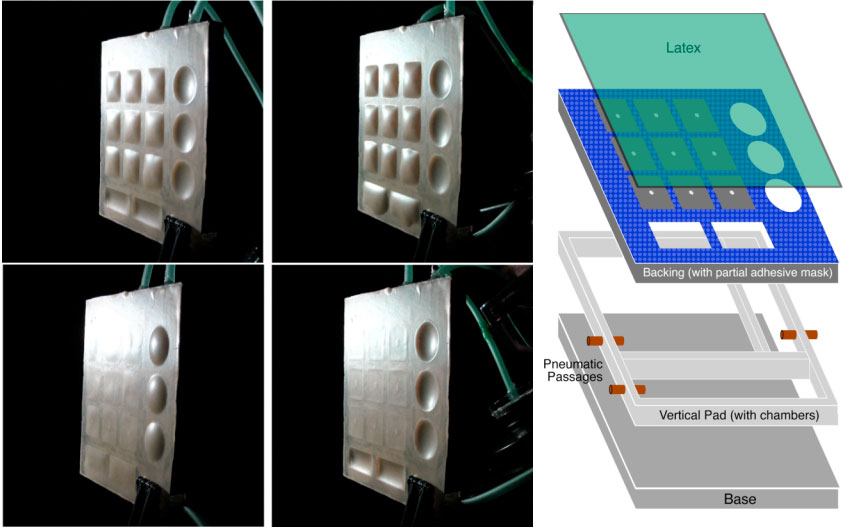
\includegraphics[width=.7\linewidth]{figures/jamming/harrisonhudson}
    \caption{A tactile display in various interface states. All buttons are statically positioned \citep{harrison2009providing}.}
    \label{fig:ch:jamming:concepts:harrisonhudson}
  \end{minipage}
\end{figure}

\paragraph{The HoverMesh (\citeyear{mazzone2004hovermesh})}
\label{ch:jamming:related-work:hci:hovermesh}
\citet{mazzone2004hovermesh} did some early work on creating a deformable structure with the jamming technique. 
The HoverMesh prototype is a cell-based jamming system consisting of 3x3 grid, see figure~\ref{fig:ch:jamming:hovermesh}.
The grid is mounted on top of a cubicle which can be inflated and deflated and together with the grid it creates deformations of the surface structure.
The HoverMesh prototype is not fully implemented according to the ideas presented.
It consists only of the grid structure on top of the cubicle and does not exhibit input capabilities through vision-based techniques and haptic feedback output as intended. 

\paragraph{ClaytricSurface (\citeyear{matoba2012claytricsurface})}
\label{ch:jamming:related-work:hci:claytric}
\citet{matoba2012claytricsurface} created a flexible tabletop surface, ClaytricSurface, which serves as a sculptable display medium (see figure~\ref{fig:ch:jamming:claytric-surface}). 
The surface can be directly manipulated by hand and the stiffness can be controlled in real time by a GUI slider.
Input is detected by a depth camera from above the tabletop.
The exemplified application of ClaytricSurface is a painting application projected onto the surface from above and a user can use direct touch on the surface to draw. 
ClaytricSurface uses the basic jamming approach and demonstrates the use of a rather large jammable surface area with direct manipulation abilities.

\begin{figure}
  \centering
  \begin{minipage}[t]{.44\textwidth}
    \centering
    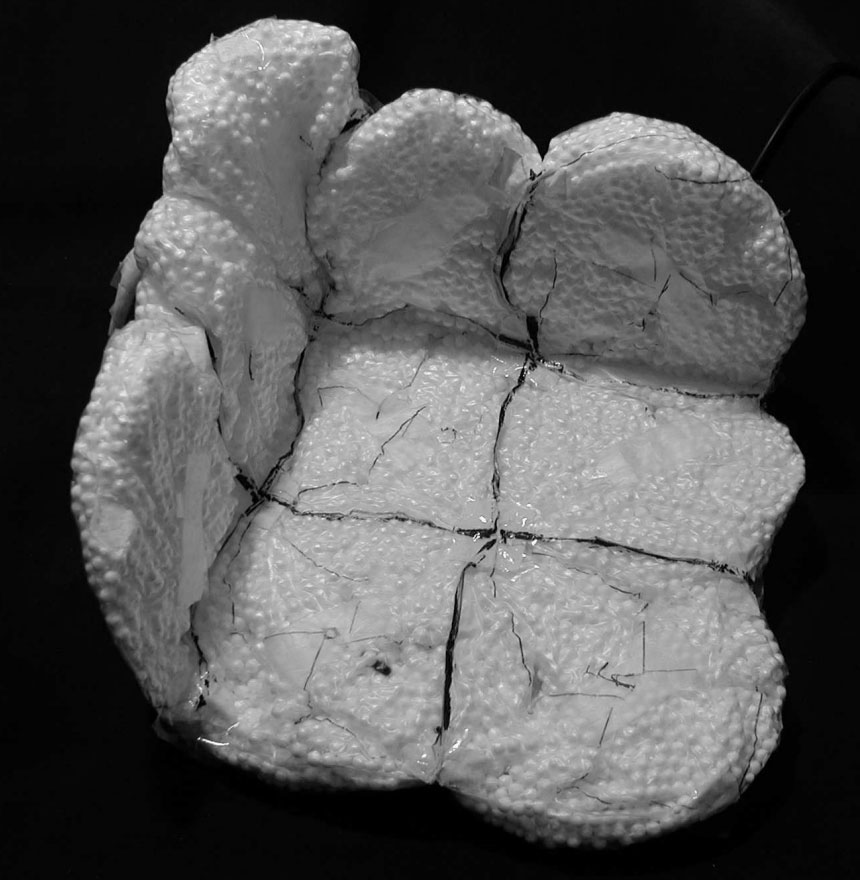
\includegraphics[width=\linewidth]{figures/jamming/hovermesh}
    \caption[The HoverMesh by \citet{mazzone2004hovermesh}.]
    {The HoverMesh \citep{mazzone2004hovermesh}.}
    \label{fig:ch:jamming:hovermesh}
  \end{minipage}%
  \hspace{0.02\textwidth}
  \begin{minipage}[t]{.44\textwidth}
    \centering
    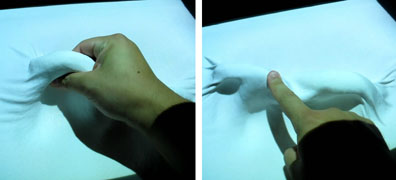
\includegraphics[width=\linewidth]{figures/jamming/claytric-surface}
    \caption[Claytric Surface by \citet{matoba2012claytricsurface}.]
    {Claytric Surface \citep{matoba2012claytricsurface}.}
    \label{fig:ch:jamming:claytric-surface}
  \end{minipage}
\end{figure}

\paragraph{Jamming User Interfaces (\citeyear{follmer2012jamming})}
\label{ch:jamming:related-work:hci:jui} 
\citet{follmer2012jamming} have probably made the biggest contribution yet to the use of jamming in HCI. 
The authors coin the approach \textit{Jamming User Interfaces} and position it in the area of malleable and organic user interfaces. 
They make several contributions to the field by exploring jamming interfaces for haptic feedback, for malleable tabletops and for mobile devices (see figure~\ref{fig:ch:jamming:jui-collection}). 
They also investigate how sensing techniques like capacitive and optical sensing, can broaden the applicability of jamming in HCI. 

\citet{follmer2012jamming} also present a hydraulic jamming system that is fast and silent and which allows for semi-transparent jamming volumes. 
This requires transparent particles, such as glass-beads, and a transparent fluid that matches the refractive index of the particles so that light refraction is reduced, see figure~\ref{fig:ch:jamming:jui:refractive}. 

\begin{figure}[h]
  \centering
  \begin{minipage}[b]{.7\textwidth}
    \centering
    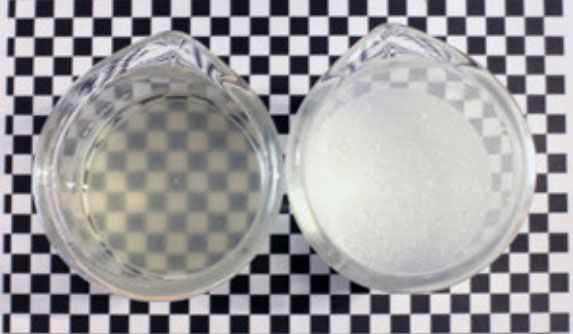
\includegraphics[width=.5\linewidth]{figures/jamming/refractive-index}
     \caption{Transparency obtained by matching the refractive index of the glass-bead particles \citep{follmer2012jamming}}.
    \label{fig:ch:jamming:jui:refractive}
  \end{minipage}
\end{figure}

In the following we will give a brief overview of the four prototypes implemented and described by \citet{follmer2012jamming}.

\subparagraph{Tunable Clay} is a malleable tabletop for direct 3D modelling (see figure~\ref{fig:ch:jamming:jui-clay}).
It resembles ClaytricSurface \citep{matoba2012claytricsurface} mentioned earlier with its clay-like surface that can easily be deformed (basic jamming approach).
Tunable Clay uses the hydraulic jamming system mentioned above with index-matched particles and fluid.
This allows for a more sophisticated depth sensing approach than the one used with ClaytricSurface.
Optical shape sensing and graphic projection is integrated underneath the jamming volume.
The shape, captured in real-time, is shown as a virtual 3D model on both an external display and on the jamming volume itself projected from underneath the surface.

\subparagraph{Transparent Haptic Lens} is a small tangible puck to be used as a haptic information channel on a tabletop display (basic jamming approach), see figure~\ref{fig:ch:jamming:jui-lens}.
It has a transparent lens in the center which is a transparent hydraulic jamming volume that can change its stiffness according to the texture beneath it.
By pressing ones finger into the lens the user can get a haptic sensation through stiffness reflecting the underlying texture of the image directly underneath. 

\subparagraph{Behind-the-Tablet Jamming} is a tablet computer which has a pneumatic jamming volume mounted on the backside (basic jamming approach), see figure~\ref{fig:ch:jamming:jui-tablet}.
The system senses malleable input with capacitive shape sensing.
The scenarios envisioned are for navigating content (e.g. scrolling and zooming) on the tablet display through malleable interaction on the backside. 
The system can communicate that some limit is reached with haptic feedback, 
e.g. by stiffening the jamming volume.

\subparagraph{ShapePhone} is a generic mobile device that can be shaped and locked into different forms (basic jamming approach).
The device has no technology inside, except for the jamming system, and it merely serves as demonstration of how its affordances change when it is sculpted into forms resembling e.g. a phone, a remote control or a watch (see figure~\ref{fig:ch:jamming:jui-phone}).
Ideas are presented for integrating various sensing techniques such as capacitive shape sensing and touch sensing to derive contextual information.

\begin{figure}
        \centering
        \begin{subfigure}[b]{0.44\textwidth}
                \centering
                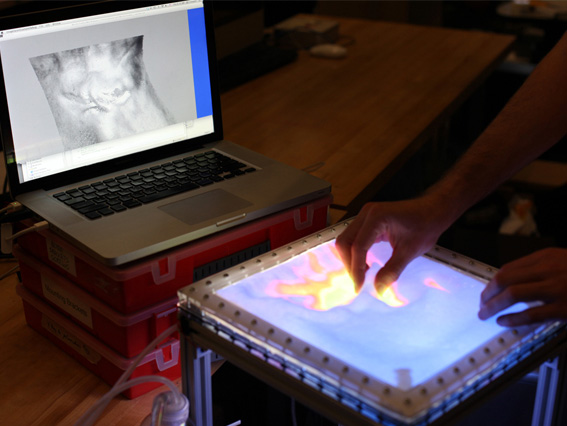
\includegraphics[width=\textwidth]{figures/jamming/jui_tunable-clay}
                \caption{Tuneable Clay}
                \label{fig:ch:jamming:jui-clay}
        \end{subfigure}
        \hspace{0.02\textwidth}
        \begin{subfigure}[b]{0.44\textwidth}
                \centering
                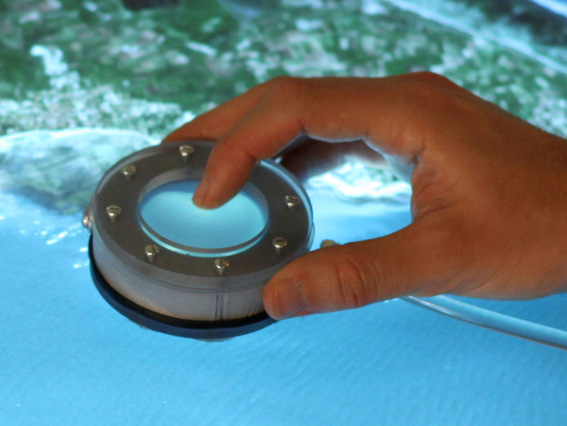
\includegraphics[width=\textwidth]{figures/jamming/jui_haptic-lens}
                \caption{Transparent Haptic Lens}
                \label{fig:ch:jamming:jui-lens}
        \end{subfigure}

        \begin{subfigure}[b]{0.44\textwidth}
                \centering
                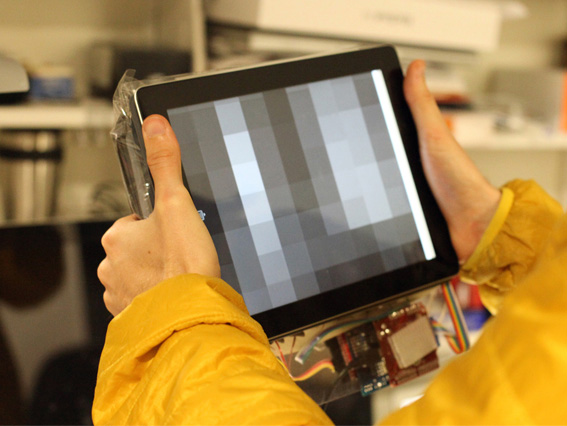
\includegraphics[width=\textwidth]{figures/jamming/jui_behind-the-tablet}
                \caption{Behind-the-Tablet Jamming}
                \label{fig:ch:jamming:jui-tablet}
        \end{subfigure}
        \hspace{0.02\textwidth}
        \begin{subfigure}[b]{0.44\textwidth}
                \centering
                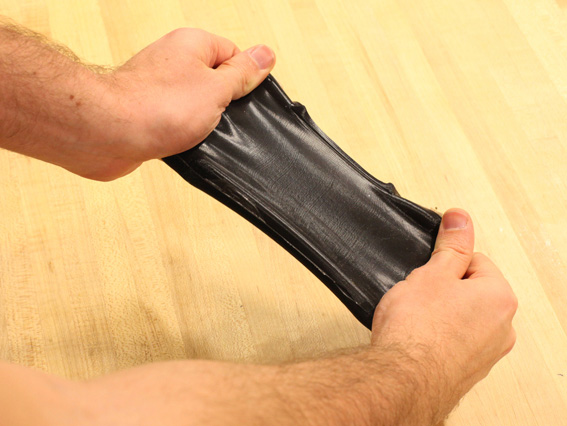
\includegraphics[width=\textwidth]{figures/jamming/jui_shapephone}
                \caption{ShapePhone}
                \label{fig:ch:jamming:jui-phone}
        \end{subfigure}
        \caption{Jamming User Interfaces by \citet{follmer2012jamming}.}
        \label{fig:ch:jamming:jui-collection}
\end{figure}

\subsection{Summary of related work}

In the previous sections we have given an introduction to the mechanics of jamming and an overview of different research applications of jamming.
These applications show two primary approaches to jamming.
The first one is the basic approach where a single volume containing particles can be jammed by applying a vacuum inside (see figure~\ref{fig:ch:jamming:approaches:basic}).
Applications of the basic approach are for example the \emph{Claytric Surface} and \emph{ShapePhone}.
The other is the more complicated cell-based approach where each cell is an independent jammable volume working in the same manner as the basic approach.
As the cells exist on the perimeter of the volume some other compound must constitute the body of the volume and stabilise the form.
In \emph{The HoverMesh} this was air inside a cubicle and in \emph{JSEL} it was fluid (see figure~\ref{fig:ch:jamming:approaches:cell}).

The related work demonstrate different potentials for the use of jamming through implementations based on mechanics, direct manipulation, shape-change, and as a feedback channel.
In table \ref{ch:jamming:table:applications_overview} we have summarises and categorises the mentioned applications according to their characteristics.
In the next section we will move on to our own concepts that support the notion of ad hoc interfaces.

\begin{landscape}
  \thispagestyle{empty}
  \centering 
  \captionof{table}{An overview and categorisation of related jamming work}
  \label{ch:jamming:table:applications_overview} 
  \begin{tabularx}{\linewidth}{|l|c|c|c|c|c|X|}
    \hline
    Project                 & Input                         & Output                        & Type      & Particles   & Approach  & Summary \\ \hline
    \hline
    Robotic gripper         & \cellcolor{FalseColor}\xmark  & \cellcolor{TrueColor}\cmark   & pneumatic & coffee      & basic     & A universal robotic gripper \\ \hline
    Jamming Skin Enabled Locomotion & \cellcolor{FalseColor}\xmark  & \cellcolor{TrueColor}\cmark   & pneumatic & glass beads     & cell-based& A soft moving robot \\ \hline
    Jamming Modulated Unimorph & \cellcolor{FalseColor}\xmark  & \cellcolor{TrueColor}\cmark   & pneumatic & glass beads          & cell-based& A worm-like robot \\ \hline
    \hline
    The HoverMesh           & \cellcolor{FalseColor}\xmark  & \cellcolor{TrueColor}\cmark   & pneumatic & polystyrene & cell-based& A cell-based deformable surface structure . \\ \hline    
    ClaytricSurface         & \cellcolor{TrueColor}\cmark   & \cellcolor{FalseColor}\xmark  & pneumatic & polystyrene & basic     & A flexible tabletop surface which serves as a sculptable display medium. \\ \hline
    Tunable Clay            & \cellcolor{TrueColor}\cmark   & \cellcolor{FalseColor}\xmark  & hydraulic & glass beads & basic     & A malleable tabletop for direct 3D modelling. \\ \hline
    Transparent Haptic Lens & \cellcolor{FalseColor}\xmark  & \cellcolor{TrueColor}\cmark   & hydraulic & glass beads & basic     & A small tangible puck to be used as a haptic information channel on a tabletop display. \\ \hline
    Behind-the-Tablet       & \cellcolor{TrueColor}\cmark   & \cellcolor{TrueColor}\cmark   & pneumatic & ?           & basic     & A tablet with a interactive jamming volume on the back. \\ \hline
    ShapePhone              & \cellcolor{TrueColor}\cmark   & \cellcolor{FalseColor}\xmark  & pneumatic & coffee      & basic     & a generic mobile device that can be shaped and locked into different forms. \\
    \hline
  \end{tabularx}

  \begin{flushleft}
  This table is an overview and categorisation of the prototypes presented in the papers covered in this section. It should be mentioned that in categorising \textit{input} and \textit{output} features we are only considering whether input or output is enabled using the jamming technique. For example, \textit{Tunable Clay} does have output in the form a image projection but it does not utilise the jamming technique.
  \end{flushleft}

\end{landscape}


\section{Concept}

\section{Technicalities}
\section{Discussion}
\todo{Maybe some Gaver (research through design) and (Alternatives, conceptual design proposals )}